\documentclass[onecolumn]{article}
%\usepackage{url}
%\usepackage{algorithmic}
\usepackage[a4paper]{geometry}
\usepackage{datetime}
\usepackage[margin=2em, font=small,labelfont=it]{caption}
\usepackage{graphicx}
\usepackage{mathpazo} % use palatino
\usepackage[scaled]{helvet} % helvetica
\usepackage{microtype}
\usepackage{amsmath}
\usepackage{subfigure}
\usepackage{listings}
\usepackage{float}
\usepackage{color} %red, green, blue, yellow, cyan, magenta, black, white
\usepackage{graphicx}
\usepackage[font=small,labelfont=bf]{caption}
\renewcommand{\thefigure}{\arabic{section}.\arabic{figure}}
\graphicspath{ {pictures/} }
\definecolor{mygreen}{RGB}{28,172,0} % color values Red, Green, Blue
\definecolor{lightgray}{gray}{0.9}
\definecolor{mylilas}{RGB}{170,55,241}
\newcommand{\inlinecode}[2]{\colorbox{lightgray}{\lstinline[language=#1]$#2$}}


% Letterspacing macros
\newcommand{\spacecaps}[1]{\textls[200]{\MakeUppercase{#1}}}
\newcommand{\spacesc}[1]{\textls[50]{\textsc{\MakeLowercase{#1}}}}

\title{\spacecaps{Lab report: Lab 1-2 }\\
Simulation of Brownian motion\\\normalsize \spacesc{Modeling of Physical Systems} }

\author{Patryk Gałczyński}
%\date{\today\\\currenttime}
\date{\today}


\begin{document}

\lstset{language=Matlab,%
    %basicstyle=\color{red},
    %breaklines=true,%
    morekeywords={matlab2tikz},
    keywordstyle=\color{blue},%
    morekeywords=[2]{1}, keywordstyle=[2]{\color{black}},
    identifierstyle=\color{black},%
    stringstyle=\color{mylilas},
    commentstyle=\color{mygreen},%
    showstringspaces=false,%without this there will be a symbol in the places where there is a space
    numbers=left,%
    numberstyle={\small \color{black}},% size of the numbers
    numbersep=9pt, % this defines how far the numbers are from the text
    emph=[1]{for,end,break},emphstyle=[1]\color{red}, %some words to emphasise
    %emph=[2]{word1,word2}, emphstyle=[2]{style},    
}

\maketitle

\begin{abstract}
This report consist specification for provided solution to given problem of simulation and analysis of Brownian motion. It describes tools used to properly simulate and visualize this physical phenomenon (MATLAB) as well as statistical operations needed to prove correctness of developed model such as autocorrelation or square mean of displacement.   
\end{abstract}


\section{Aim}
\large
The aim of this laboratory was to simulate and analyze Brownian motion and its properties using various selected methods. 


\section{Methods}
For the laboratory purpose various tools and methods were selected to achieve good simulation results and easy in depth analysis.

\subsection{Software}
To simulate, compute and visually represent Brownian motion MATLAB software were involved.
\subsection{Statistical methods}
\begin{itemize}
	\item A random walk model was used for good approximation of Brownian motion;
    \item A mean square of displacement was used to measure spatial extent of particle;
    \item A autocorrelation was used to show property named as ``self similarity'';
    \item A histogram of particle position to illustrate the time evolution of particles density.
\end{itemize}

\section{Results}
\subsection{simulating Brownian motion}
To simulate Brownian motion, matlab function has been developed. The function does take 3 arguments, as follows: number of dimensions to carry simulation in, number of particle movements to simulate and number of particles to use.

\vspace{1em}

\begin{lstlisting}[language=Matlab,frame=single,breaklines=true,caption={Function that simulates Brownian motion}]
function [] = brownian(dims, num_of_movements, num_of_particles)
   figure;
   for i = 1:num_of_particles
       % initiaze variables
       N = num_of_movements;
       X(1) = 0;
       Y(1) = 0;
       Z(1) = 0;
       % generate random vectors
       for i=2:N
           X(i) = X(i-1) + randn();
           Y(i) = Y(i-1) + randn();
           Z(i) = Z(i-1) + randn();
       end
       % plot the result
       if dims == 1
           plot(Y);
           ylabel('x coordinate');
           xlabel('timestamp');
       elseif dims == 2
           plot(X,Y);
           xlabel('x coordinate');
           ylabel('y coordinate');
       elseif dims == 3
           plot3(X,Y,Z);
           xlabel('x coordinate');
           ylabel('y coordinate');
           zlabel('z coordinate')
       end
       hold on;
   end
end
\end{lstlisting}

\newpage
Results of this function call for different sets of arguments are shown on Figure \ref{fig:brownian}
\begin{figure}[H]
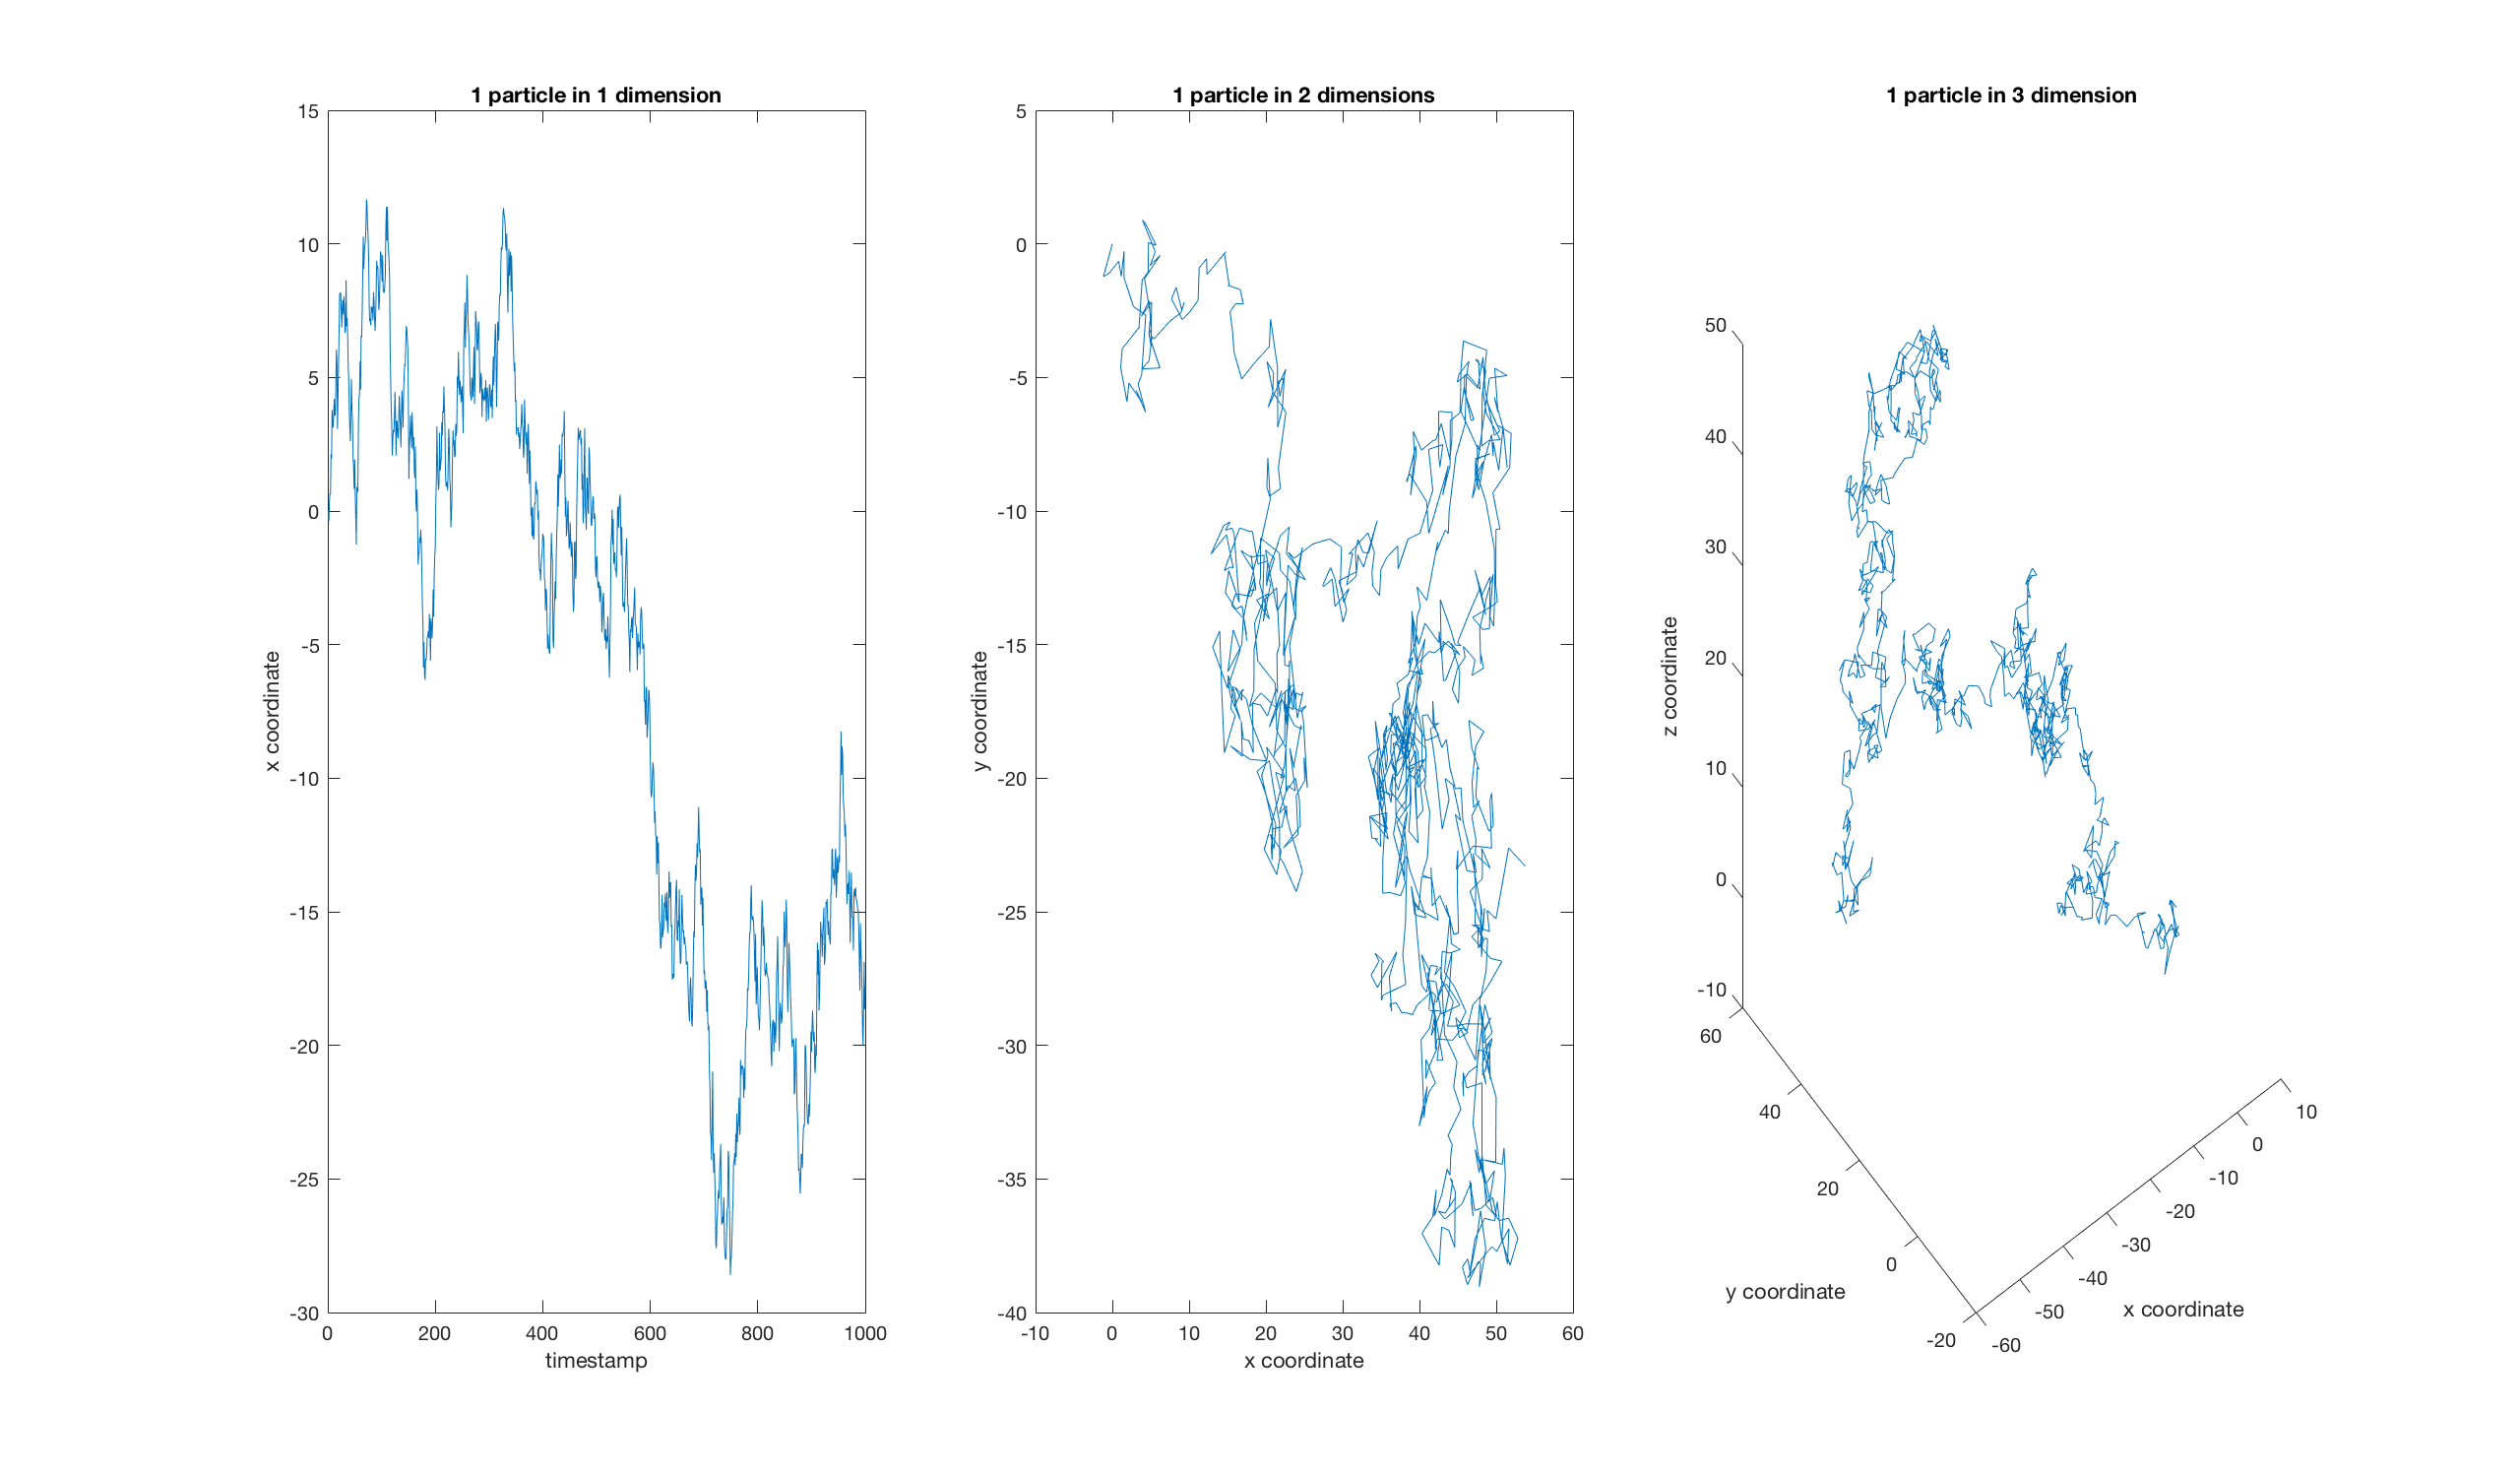
\includegraphics[width=\textwidth]{motion_1p}
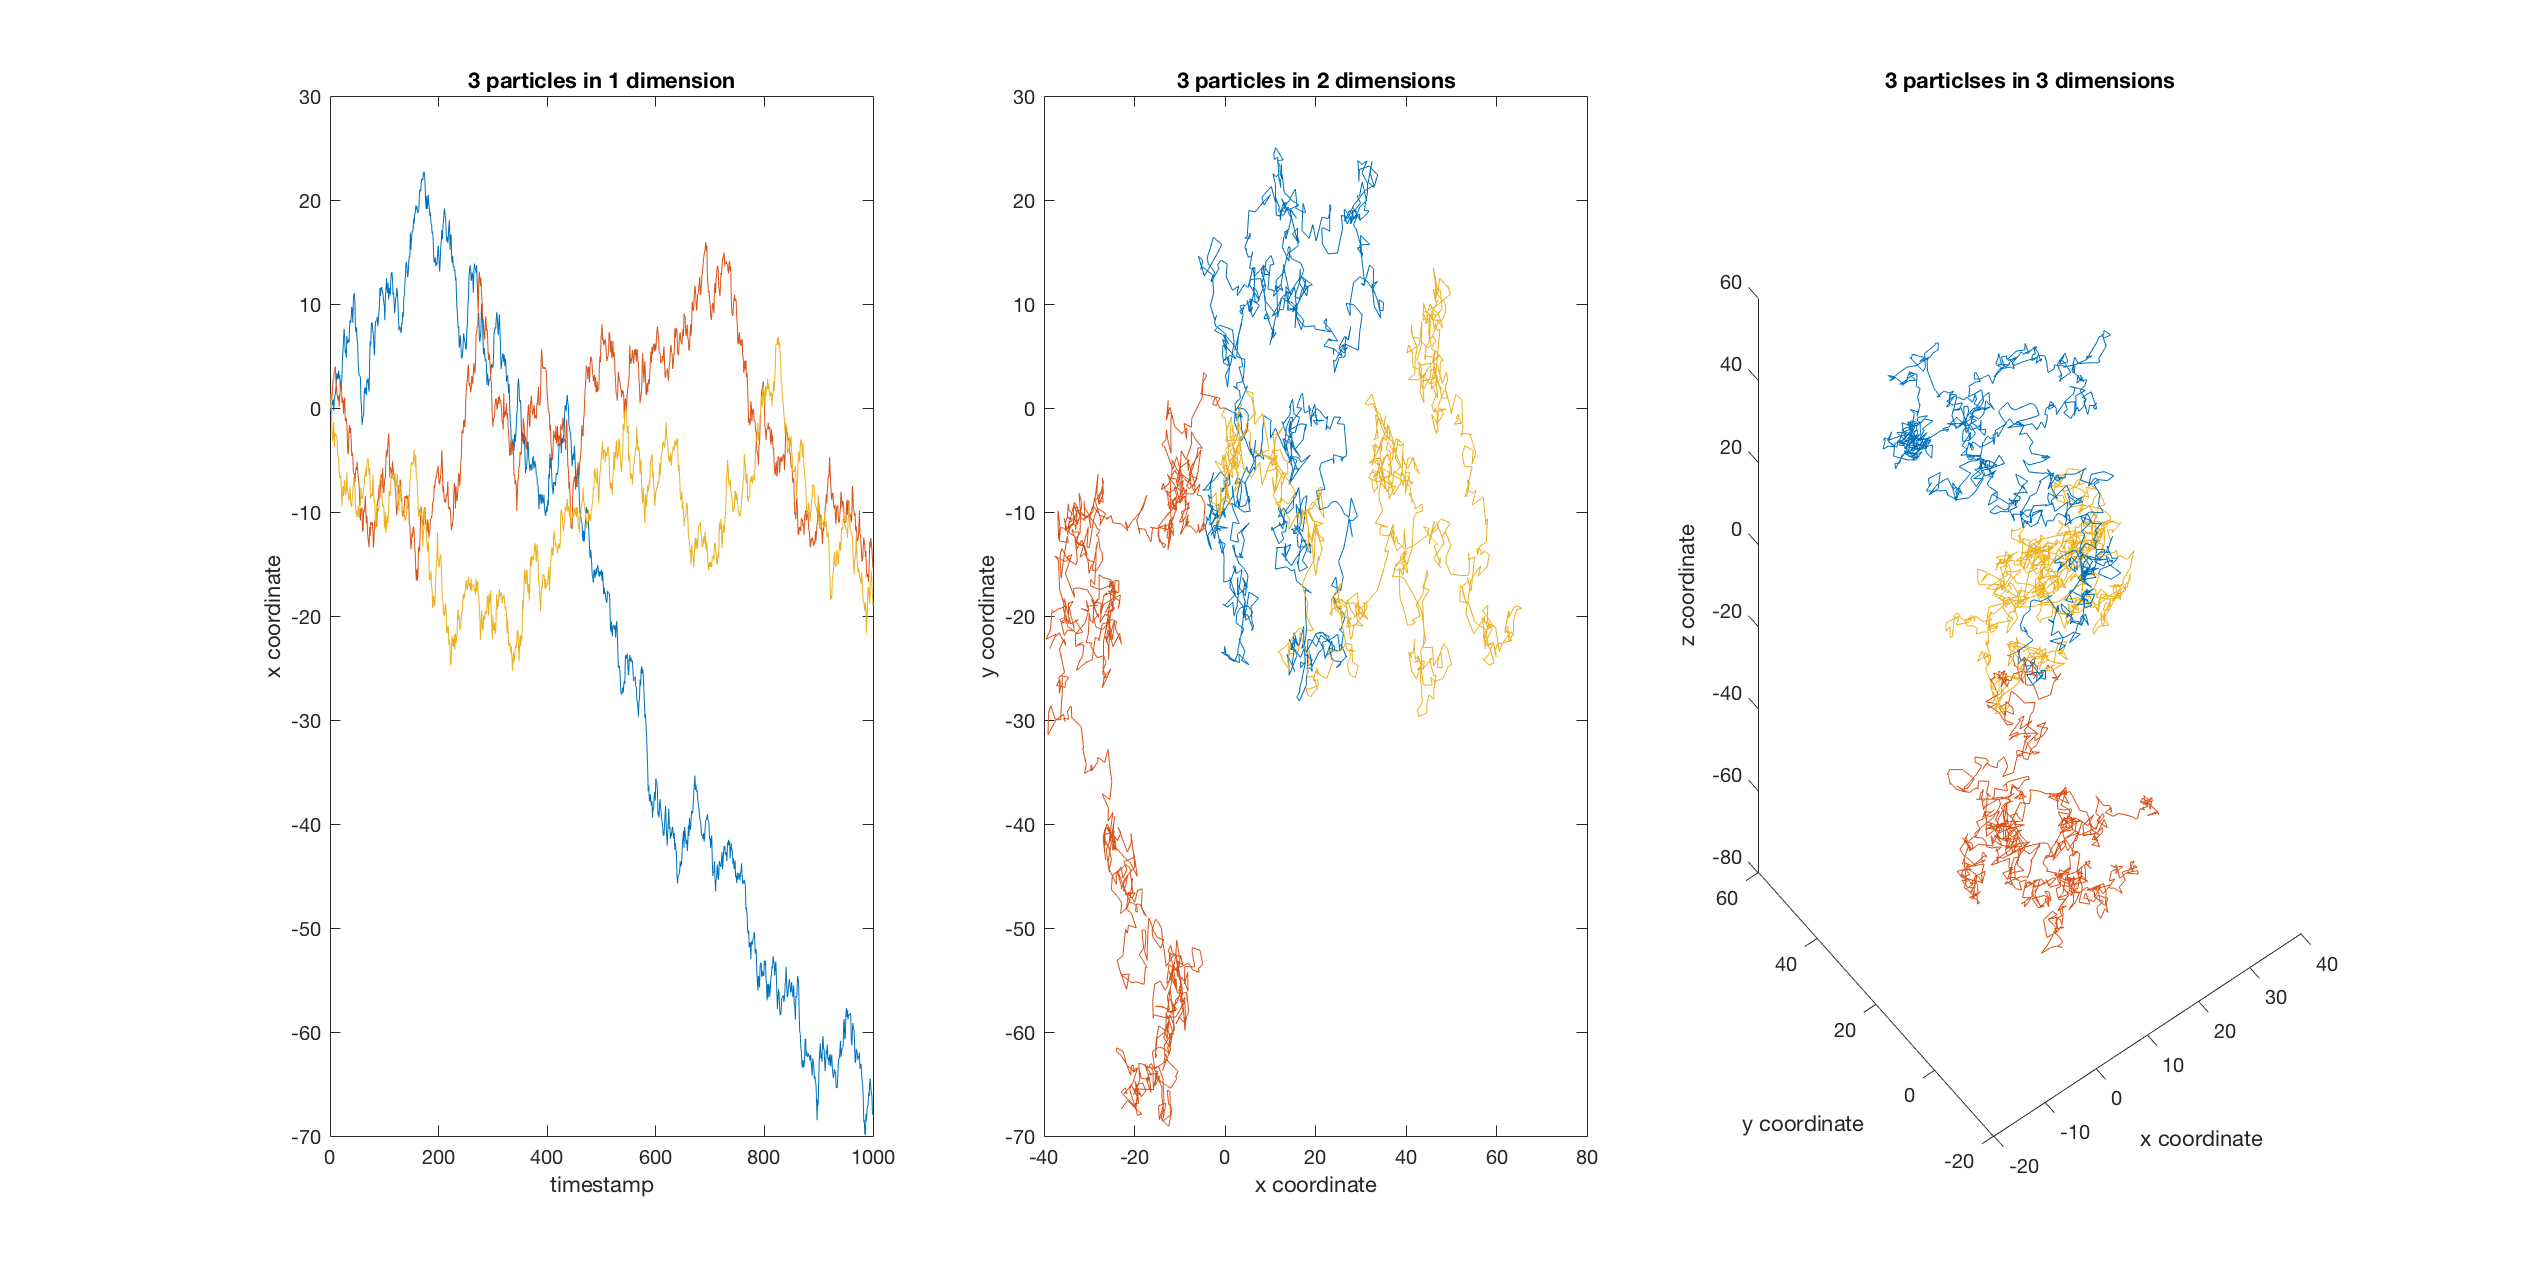
\includegraphics[width=\textwidth]{motion_3p}
\caption{Brownian motion simulation for different number of dimensions and number of particles}
\label{fig:brownian}
\end{figure}

\subsection{Square mean of displacement and time}
Mean square displacement is a measurement of how far particle goes over time from previous position (in this case). To calculate that value another MATLAB function has been written. It takes similar set of arguments as previous function and plots mean square displacement over time.

Function \inlinecode{Matlab}{square\_means} can be found on listing \ref{lst:sqare_mean}

\vspace{1em}

\begin{lstlisting}[language=Matlab,frame=single,label={lst:sqare_mean},breaklines=true,caption={Function that calculates square mean of displacement}]
function [] = square_mean(dims, num_of_movements, num_of_particles)
    N = num_of_movements;
    num_of_parts = num_of_particles;
    x = zeros(num_of_parts, 1);
    y = zeros(num_of_parts, 1);
    z = zeros(num_of_parts, 1);
    for i=2:N
       x = [x x(:,i-1)+randn(num_of_parts, 1)];
       y = [y y(:,i-1)+randn(num_of_parts, 1)];
       z = [z z(:,i-1)+randn(num_of_parts, 1)];
    end

    if dims == 1
           plot(sum(x.^2)/num_of_parts');
           xlabel('timestamp');
           ylabel('Square mean of displacement in 1d');
           title(['1 dimension for ' num2str(num_of_parts) ' particles']);
       elseif dims == 2
           plot(sum(x.^2 + y.^2)/num_of_parts');
           xlabel('timestamp');
           ylabel('Square mean of displacement in 2d');
           title(['2 dimensions for ' num2str(num_of_parts) ' particles']);
       elseif dims == 3
           plot(sum(x.^2 + y.^2 + z.^2)/num_of_parts');
           xlabel('timestamp');
           ylabel('Square mean of displacement in 3d');
           title(['3 dimensions for ' num2str(num_of_parts) ' particles']);
    end
end
\end{lstlisting}

\vspace{1em}
Output for various sets of input parameters are shown on Figures \ref{fig:1d_2d} and \ref{fig:3d}

\begin{figure}[H]
\noindent\makebox[\textwidth]{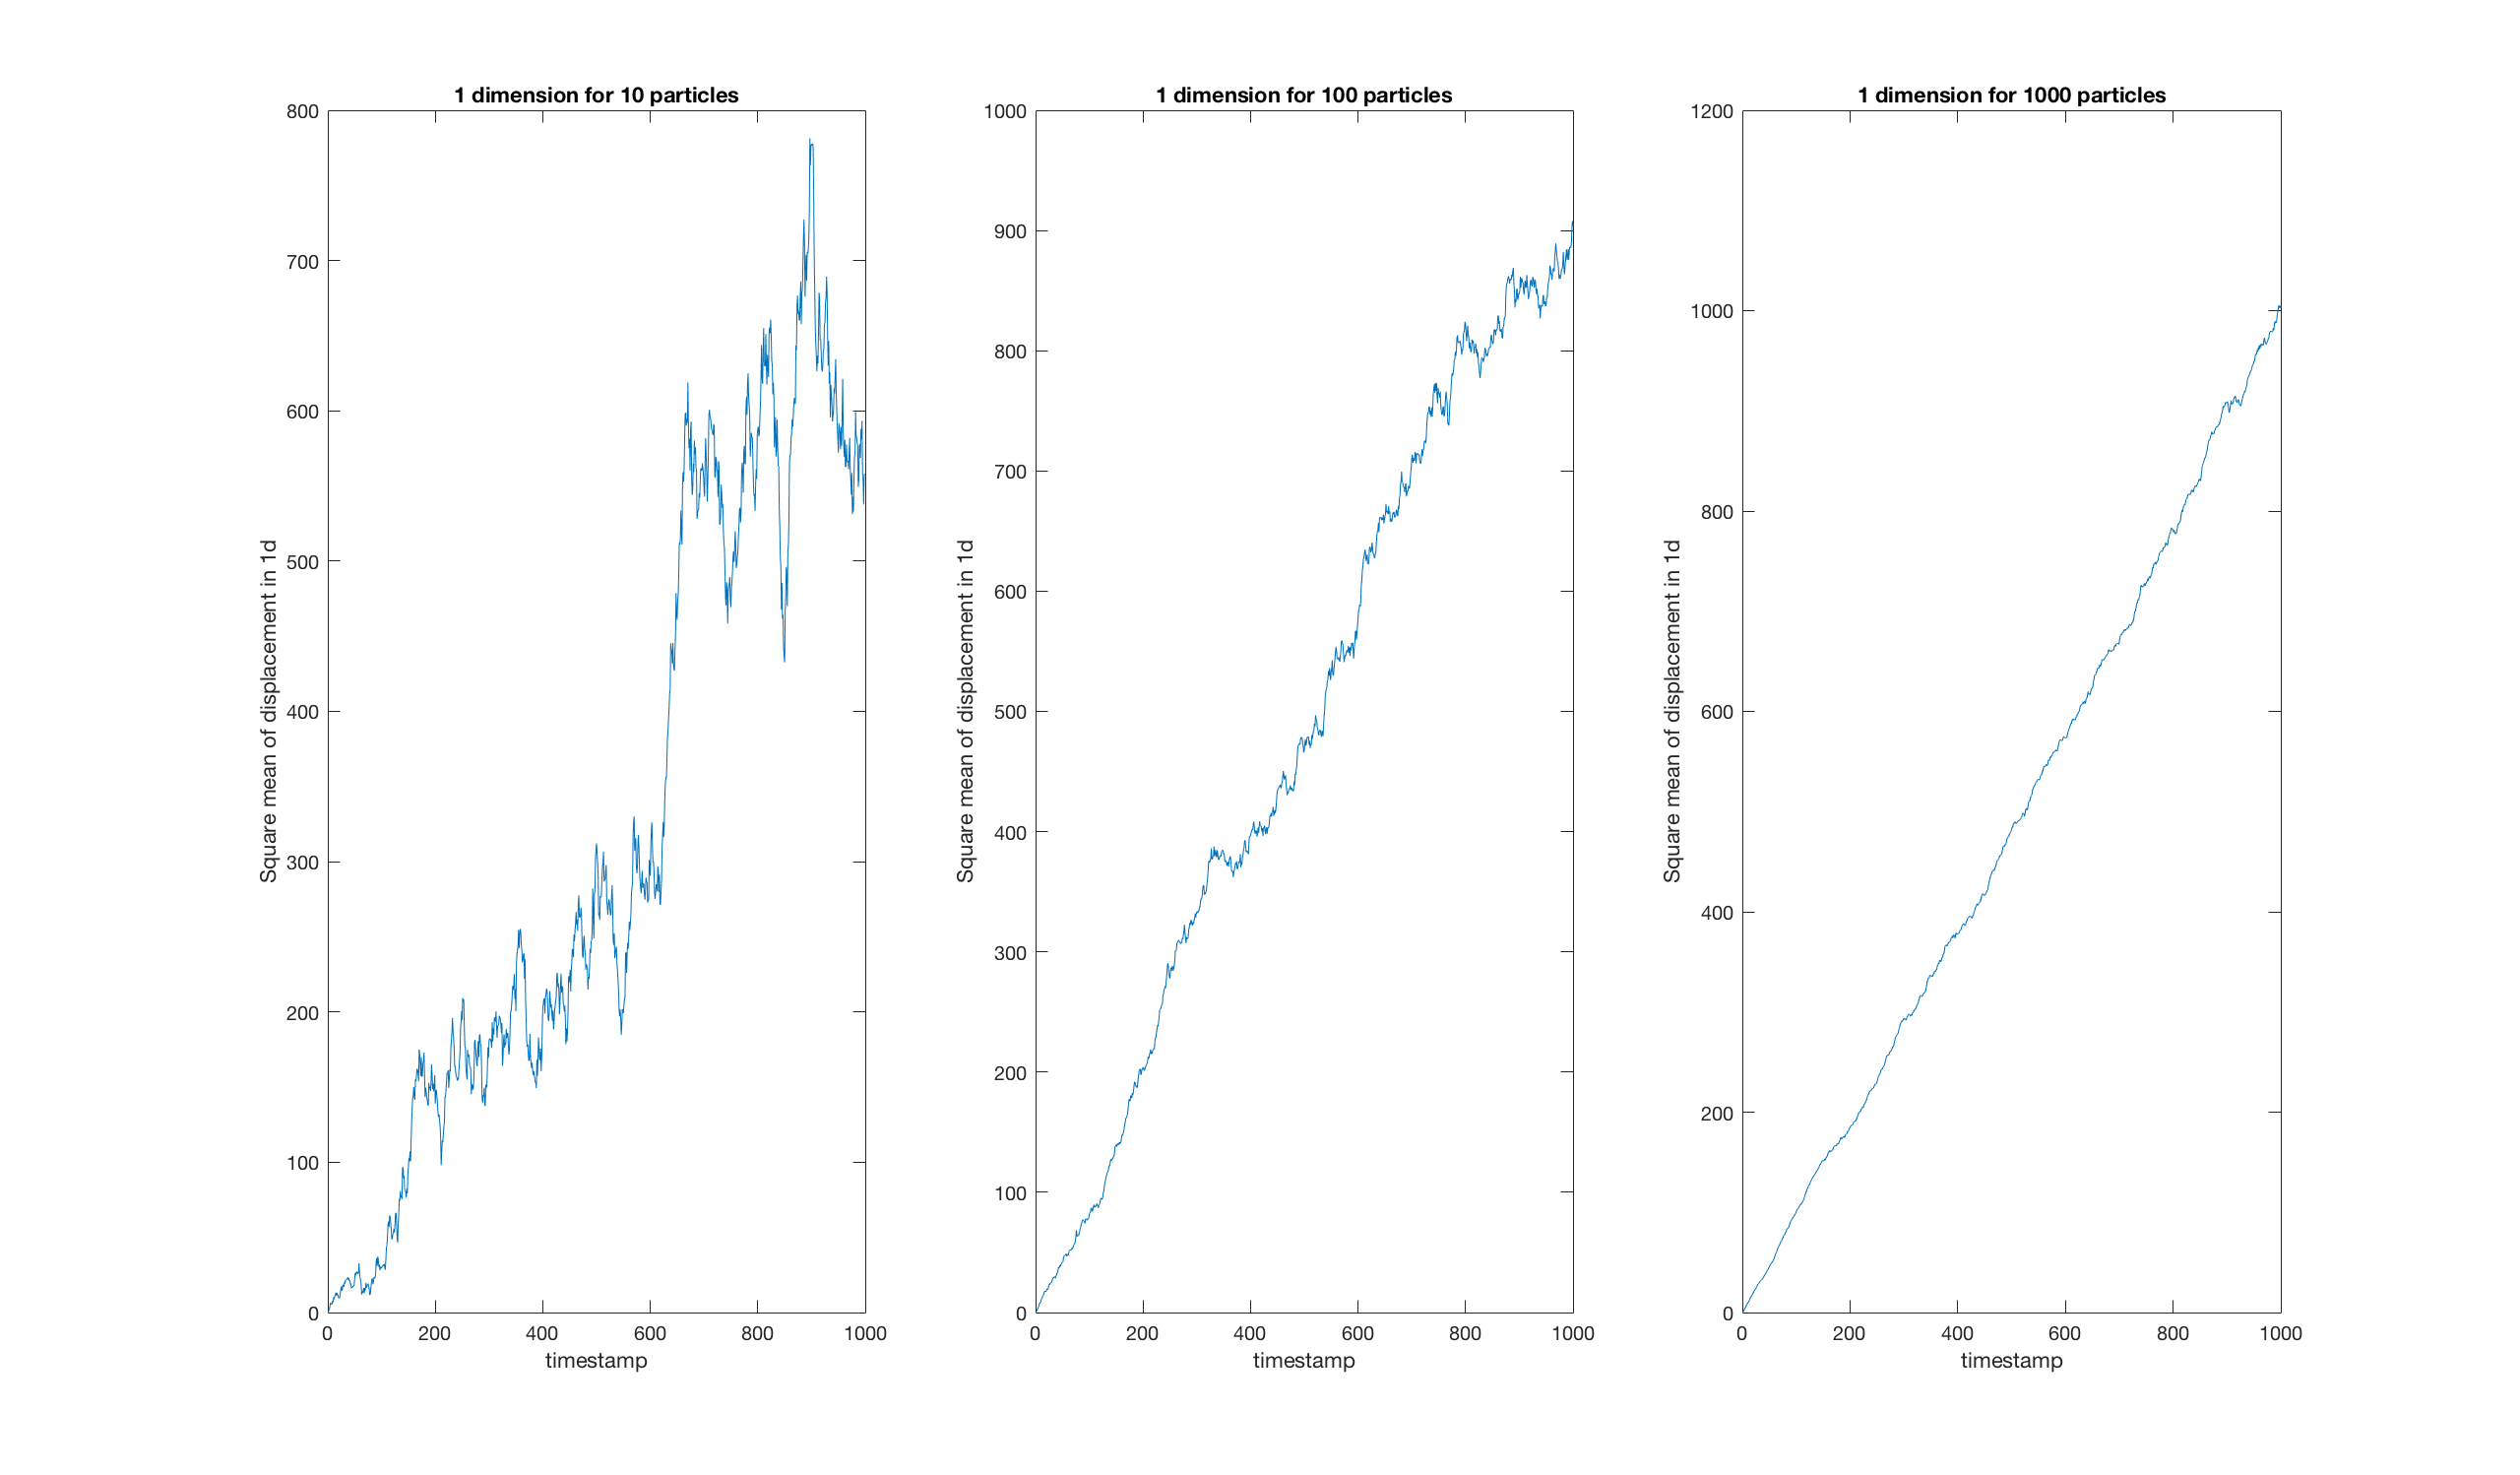
\includegraphics[width=\paperwidth,height=8cm]{smod_1d}}
\noindent\makebox[\textwidth]{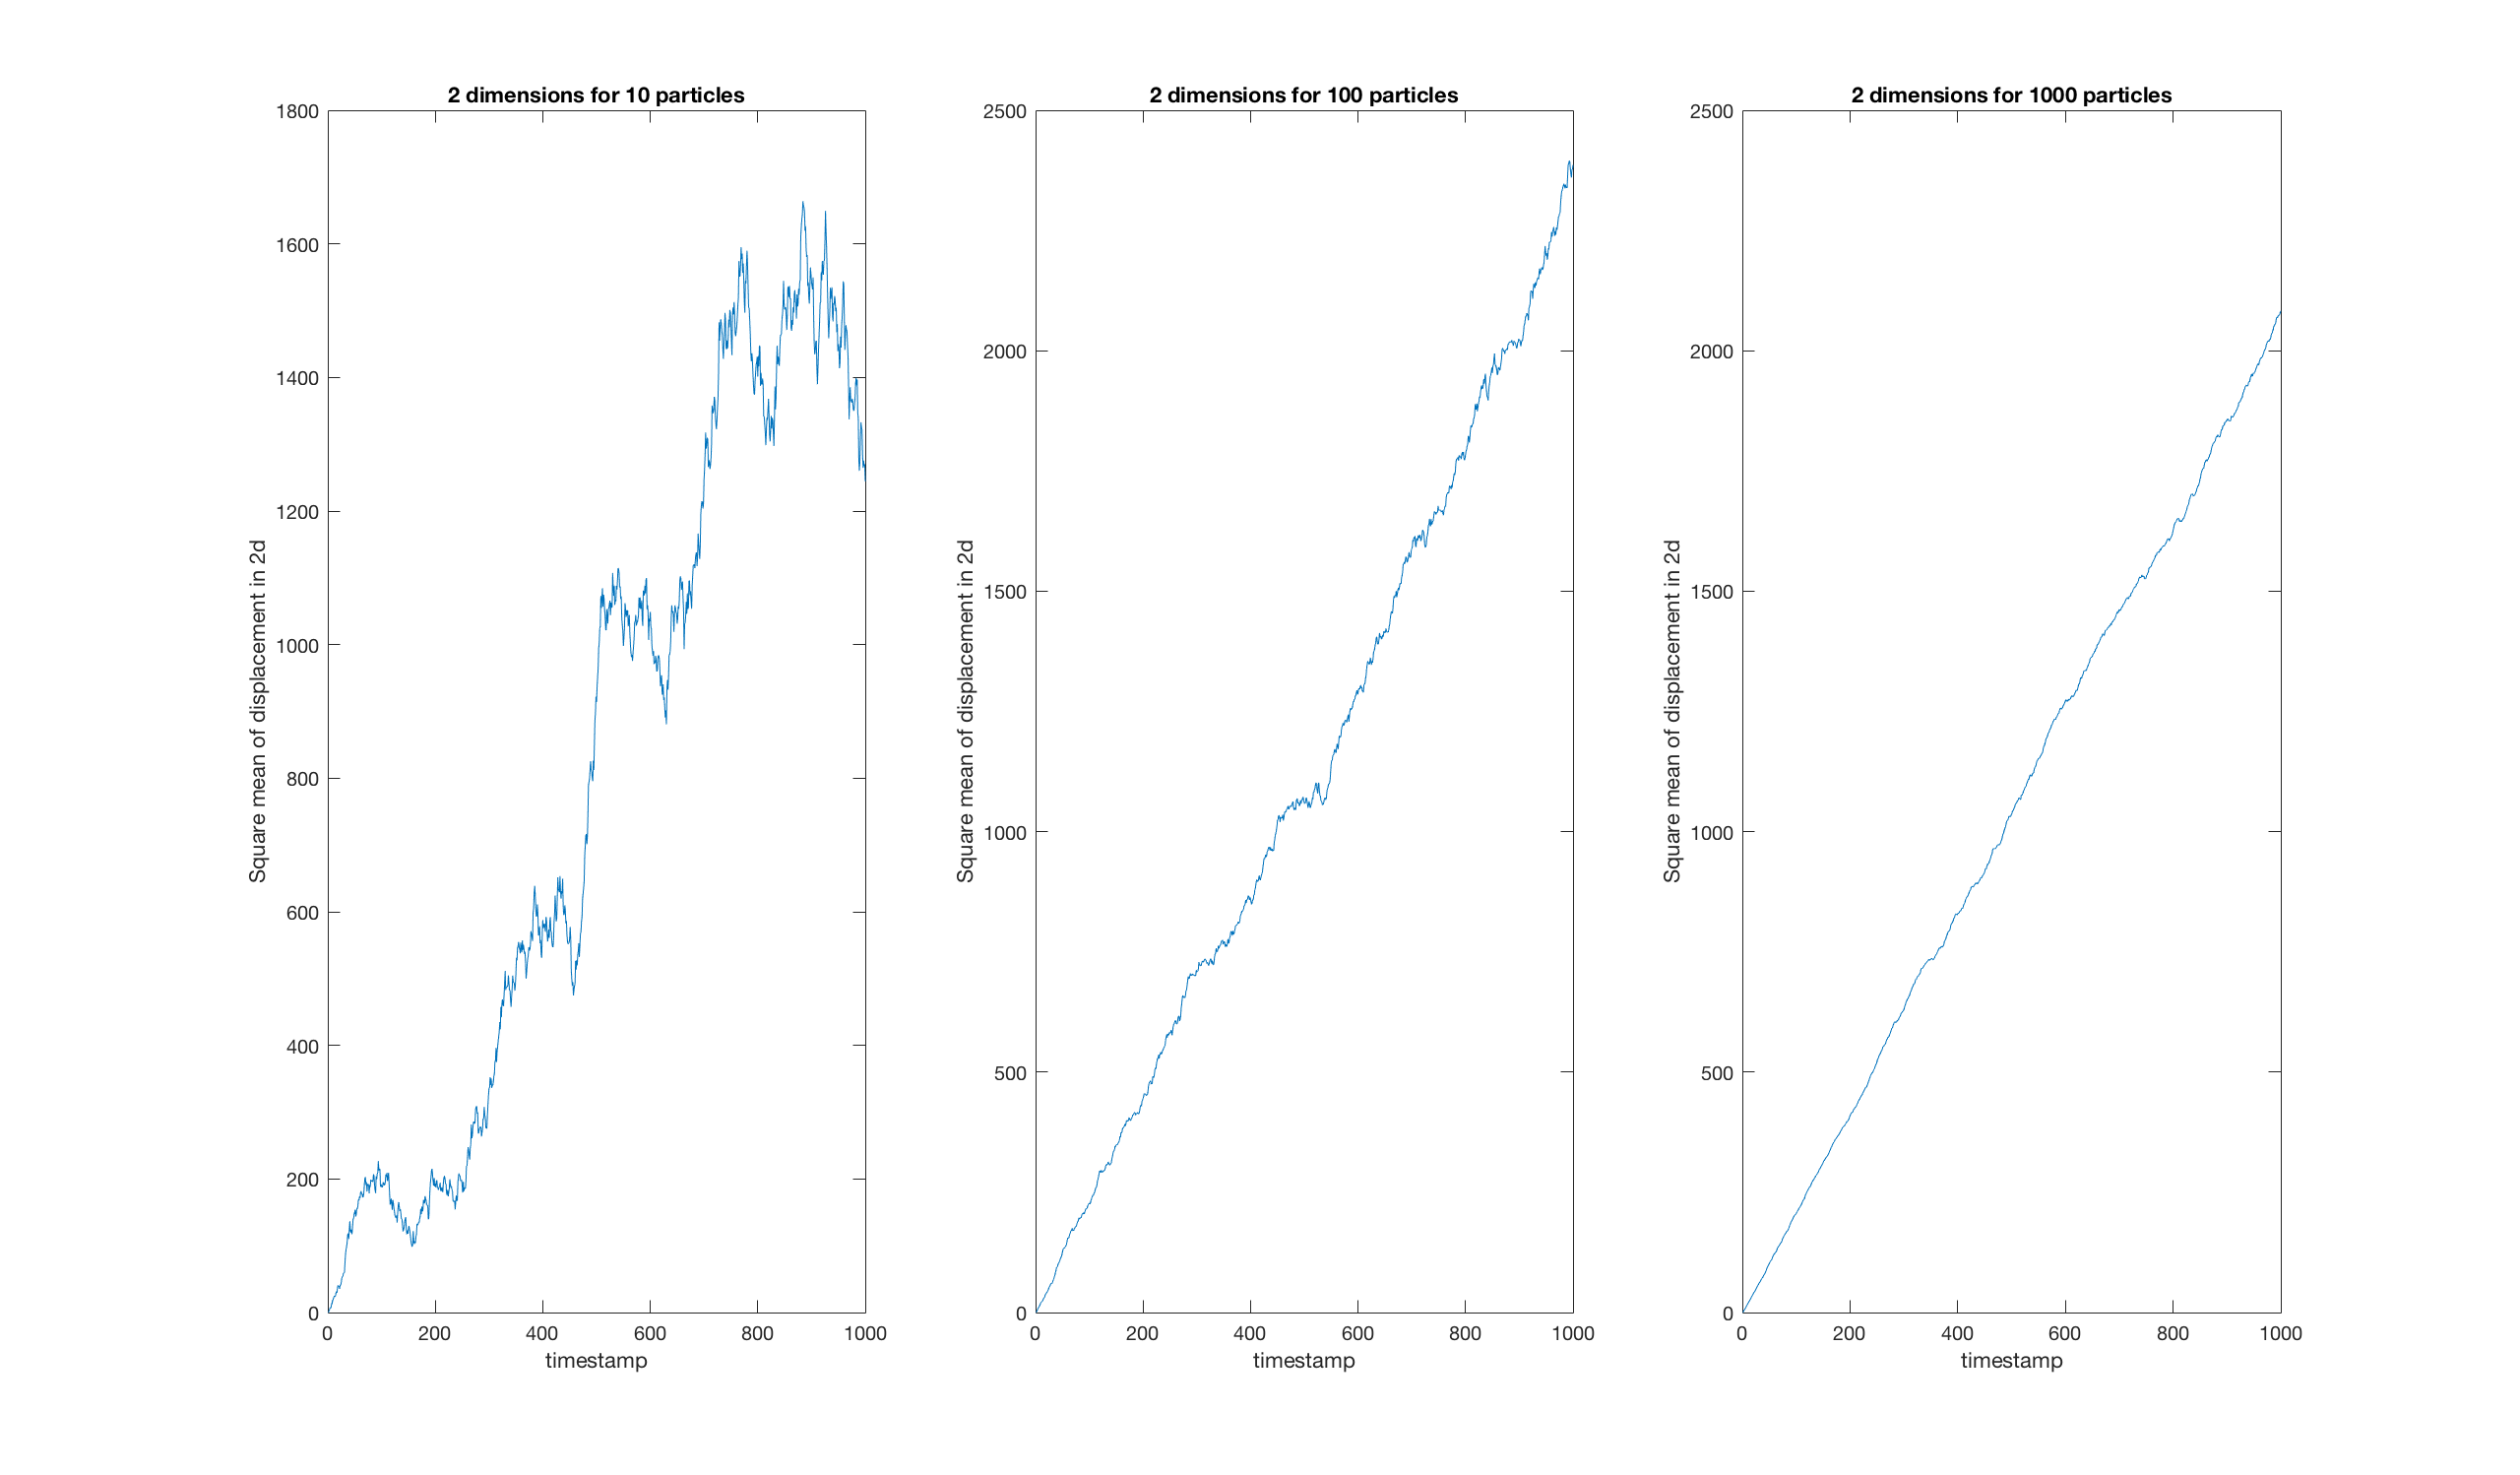
\includegraphics[width=\paperwidth,height=8cm]{smod_2d}}
\caption{Mean square displacement for various number of particles in 1d and 2d}
\label{fig:1d_2d}
\end{figure}

\begin{figure}[H]
\noindent\makebox[\textwidth]{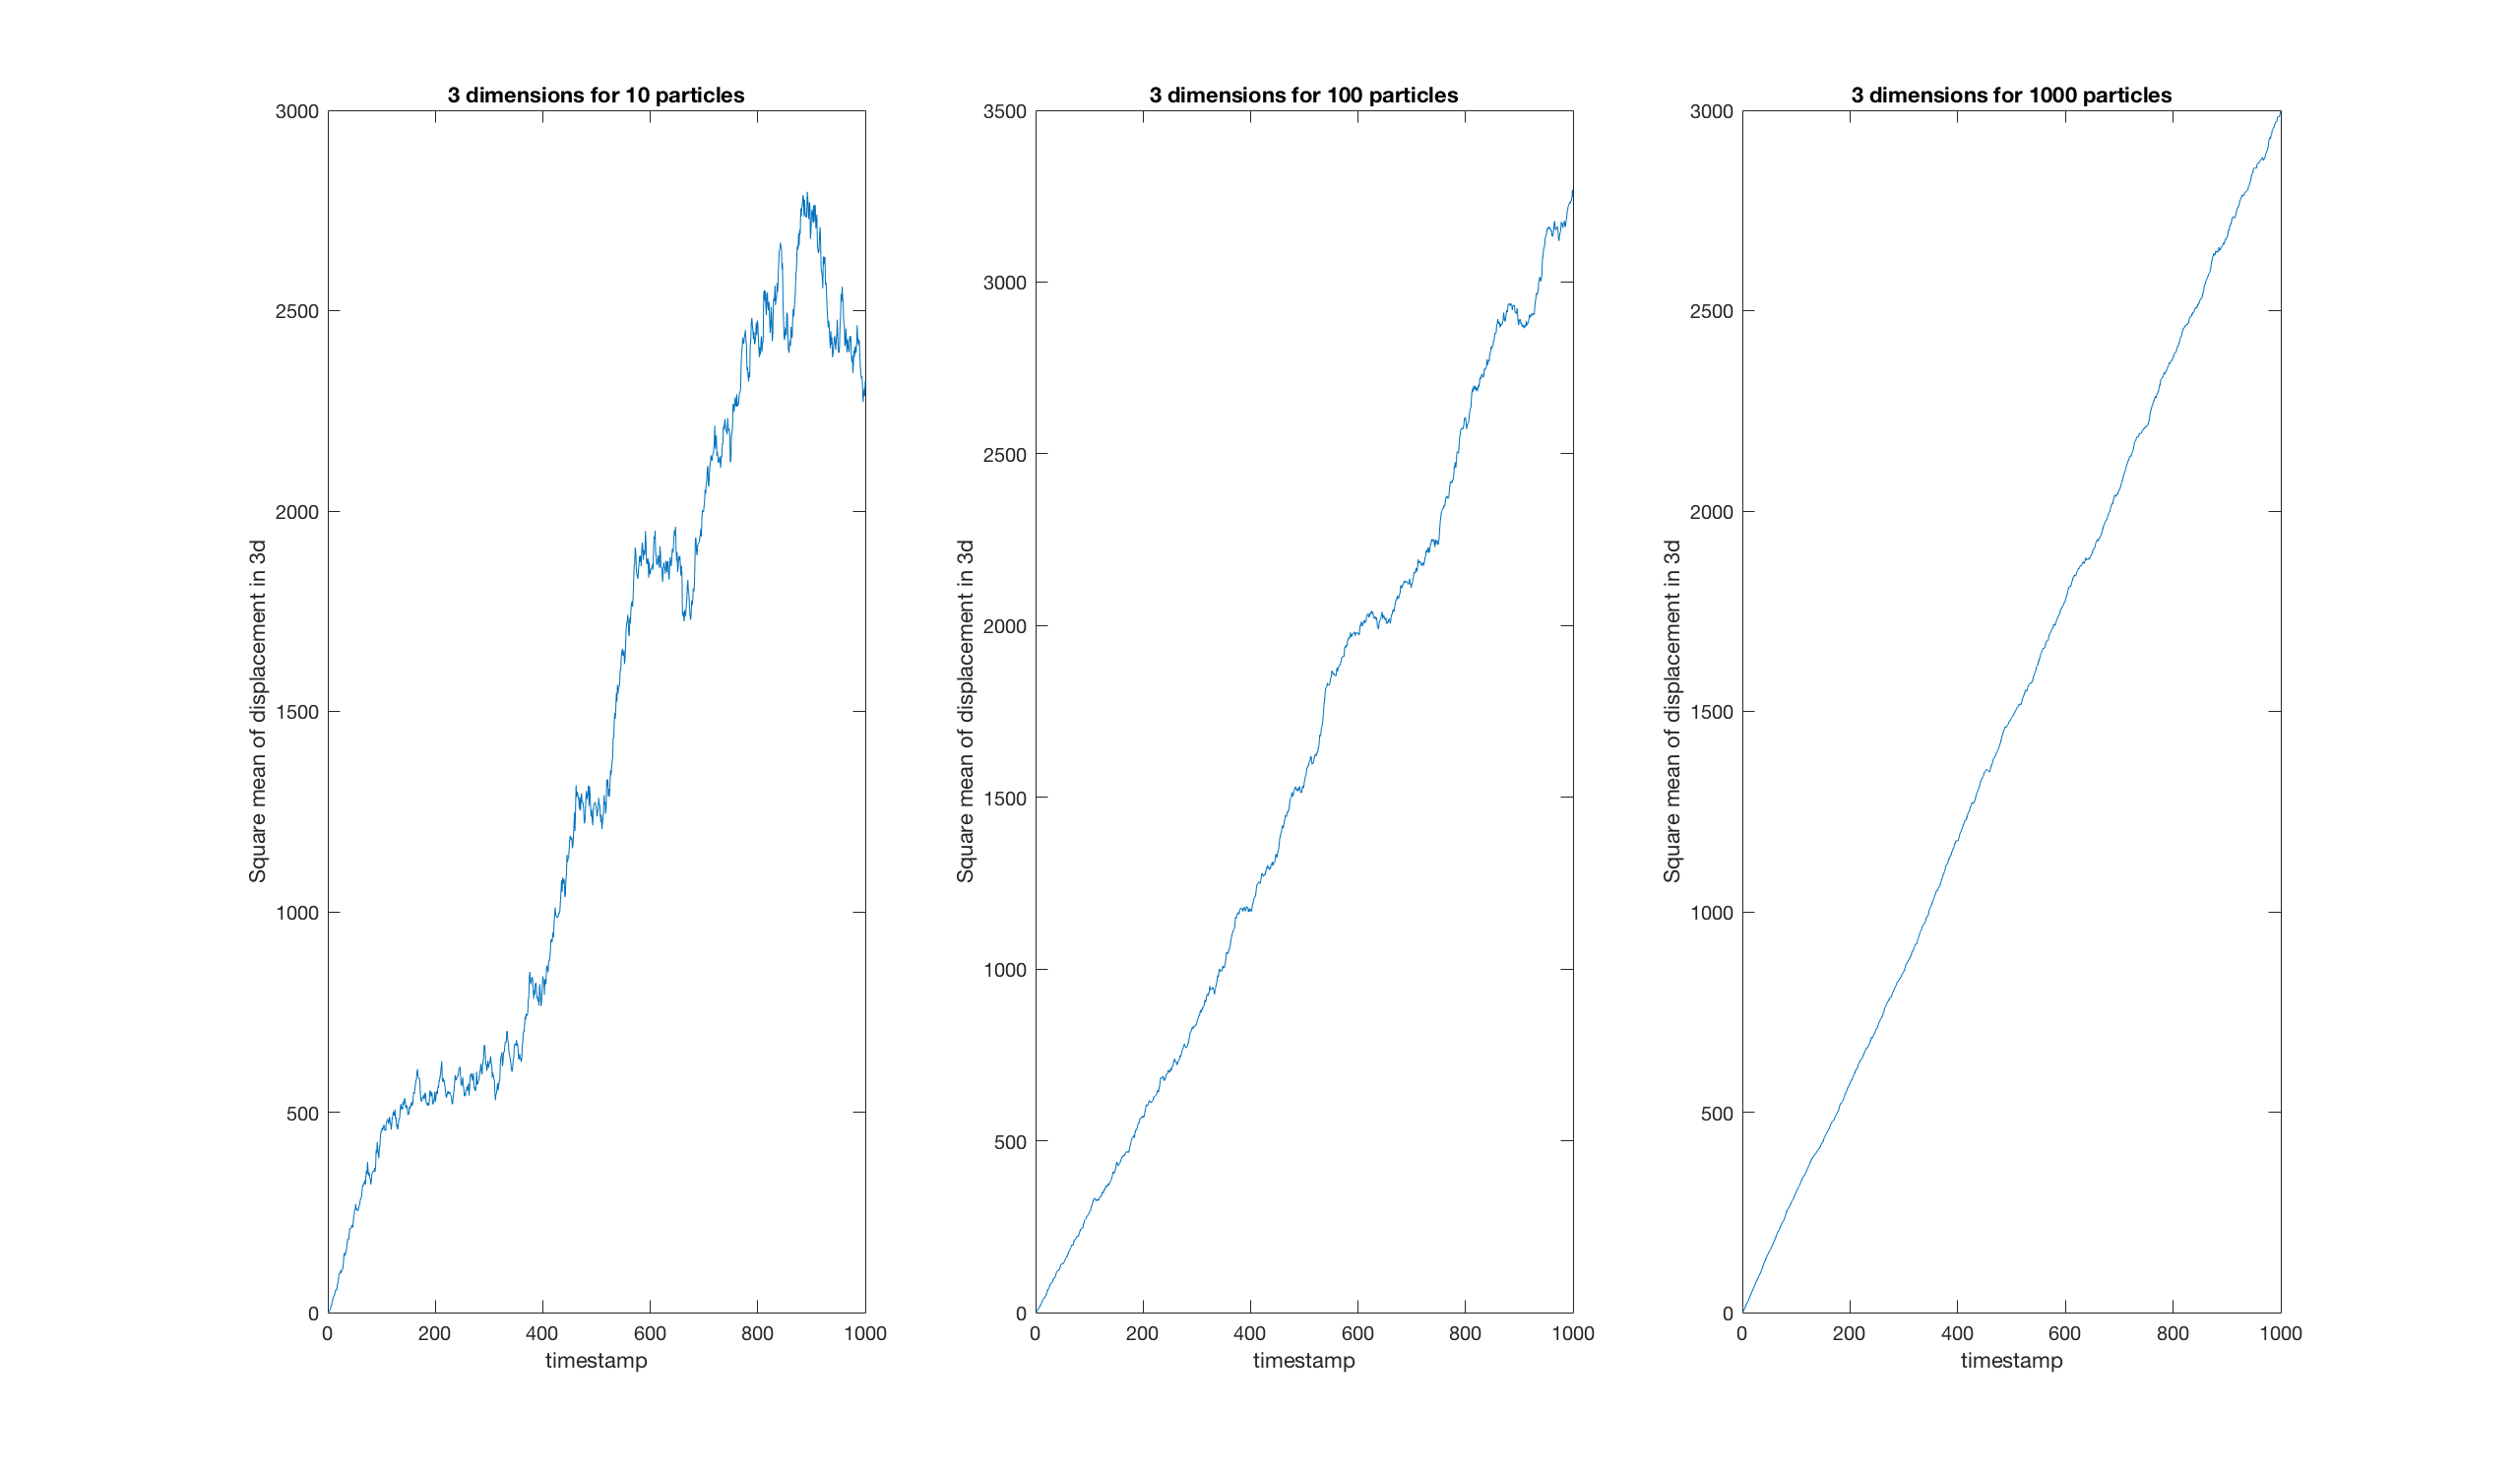
\includegraphics[width=\paperwidth,height=8cm]{smod_3d}}
\caption{Mean square displacement for various number of particles in 3d}
\label{fig:3d}
\end{figure}

From this carts, it is clearly visible that, with growing number of particles, relationship between timestamp and square mean of displacement is getting more and more linear-ish.


\subsection{Time evolution of particles density}

To demonstrate the particles density evolution over time histogram has been used. However, it is suitable only for 1d and 2d data, so only these two are going to be analyzed. Matlab code used to generate such plots is shown on Listing \ref{lst:histograms}

\vspace{1em}

\begin{lstlisting}[language=Matlab,frame=single,label={lst:histograms},breaklines=true,caption={Function that calculates particles density evolution}]
function [] = density(dims, num_of_particles)
    num_of_parts = num_of_particles;
    x = zeros(num_of_parts, 1);
    y = zeros(num_of_parts, 1);
    z = zeros(num_of_parts, 1);

    for i=2:num_of_parts
       x = [x x(:,i-1)+randn(num_of_parts, 1)];
       y = [y y(:,i-1)+randn(num_of_parts, 1)];
       z = [z z(:,i-1)+randn(num_of_parts, 1)];
    end
    
    

    if dims == 1
           figure;
           histogram(x);
           xlabel('x coordinate');
           ylabel('number of particles');
    elseif dims == 2
           figure;
           histogram2(x,y);
           xlabel('x coordinate');
           ylabel('y coordinate');
           zlabel('number of particles');
    end
end
\end{lstlisting}

\vspace{1em}

Such code execution gave following results:

\begin{figure}[H]
\noindent\makebox[\textwidth]{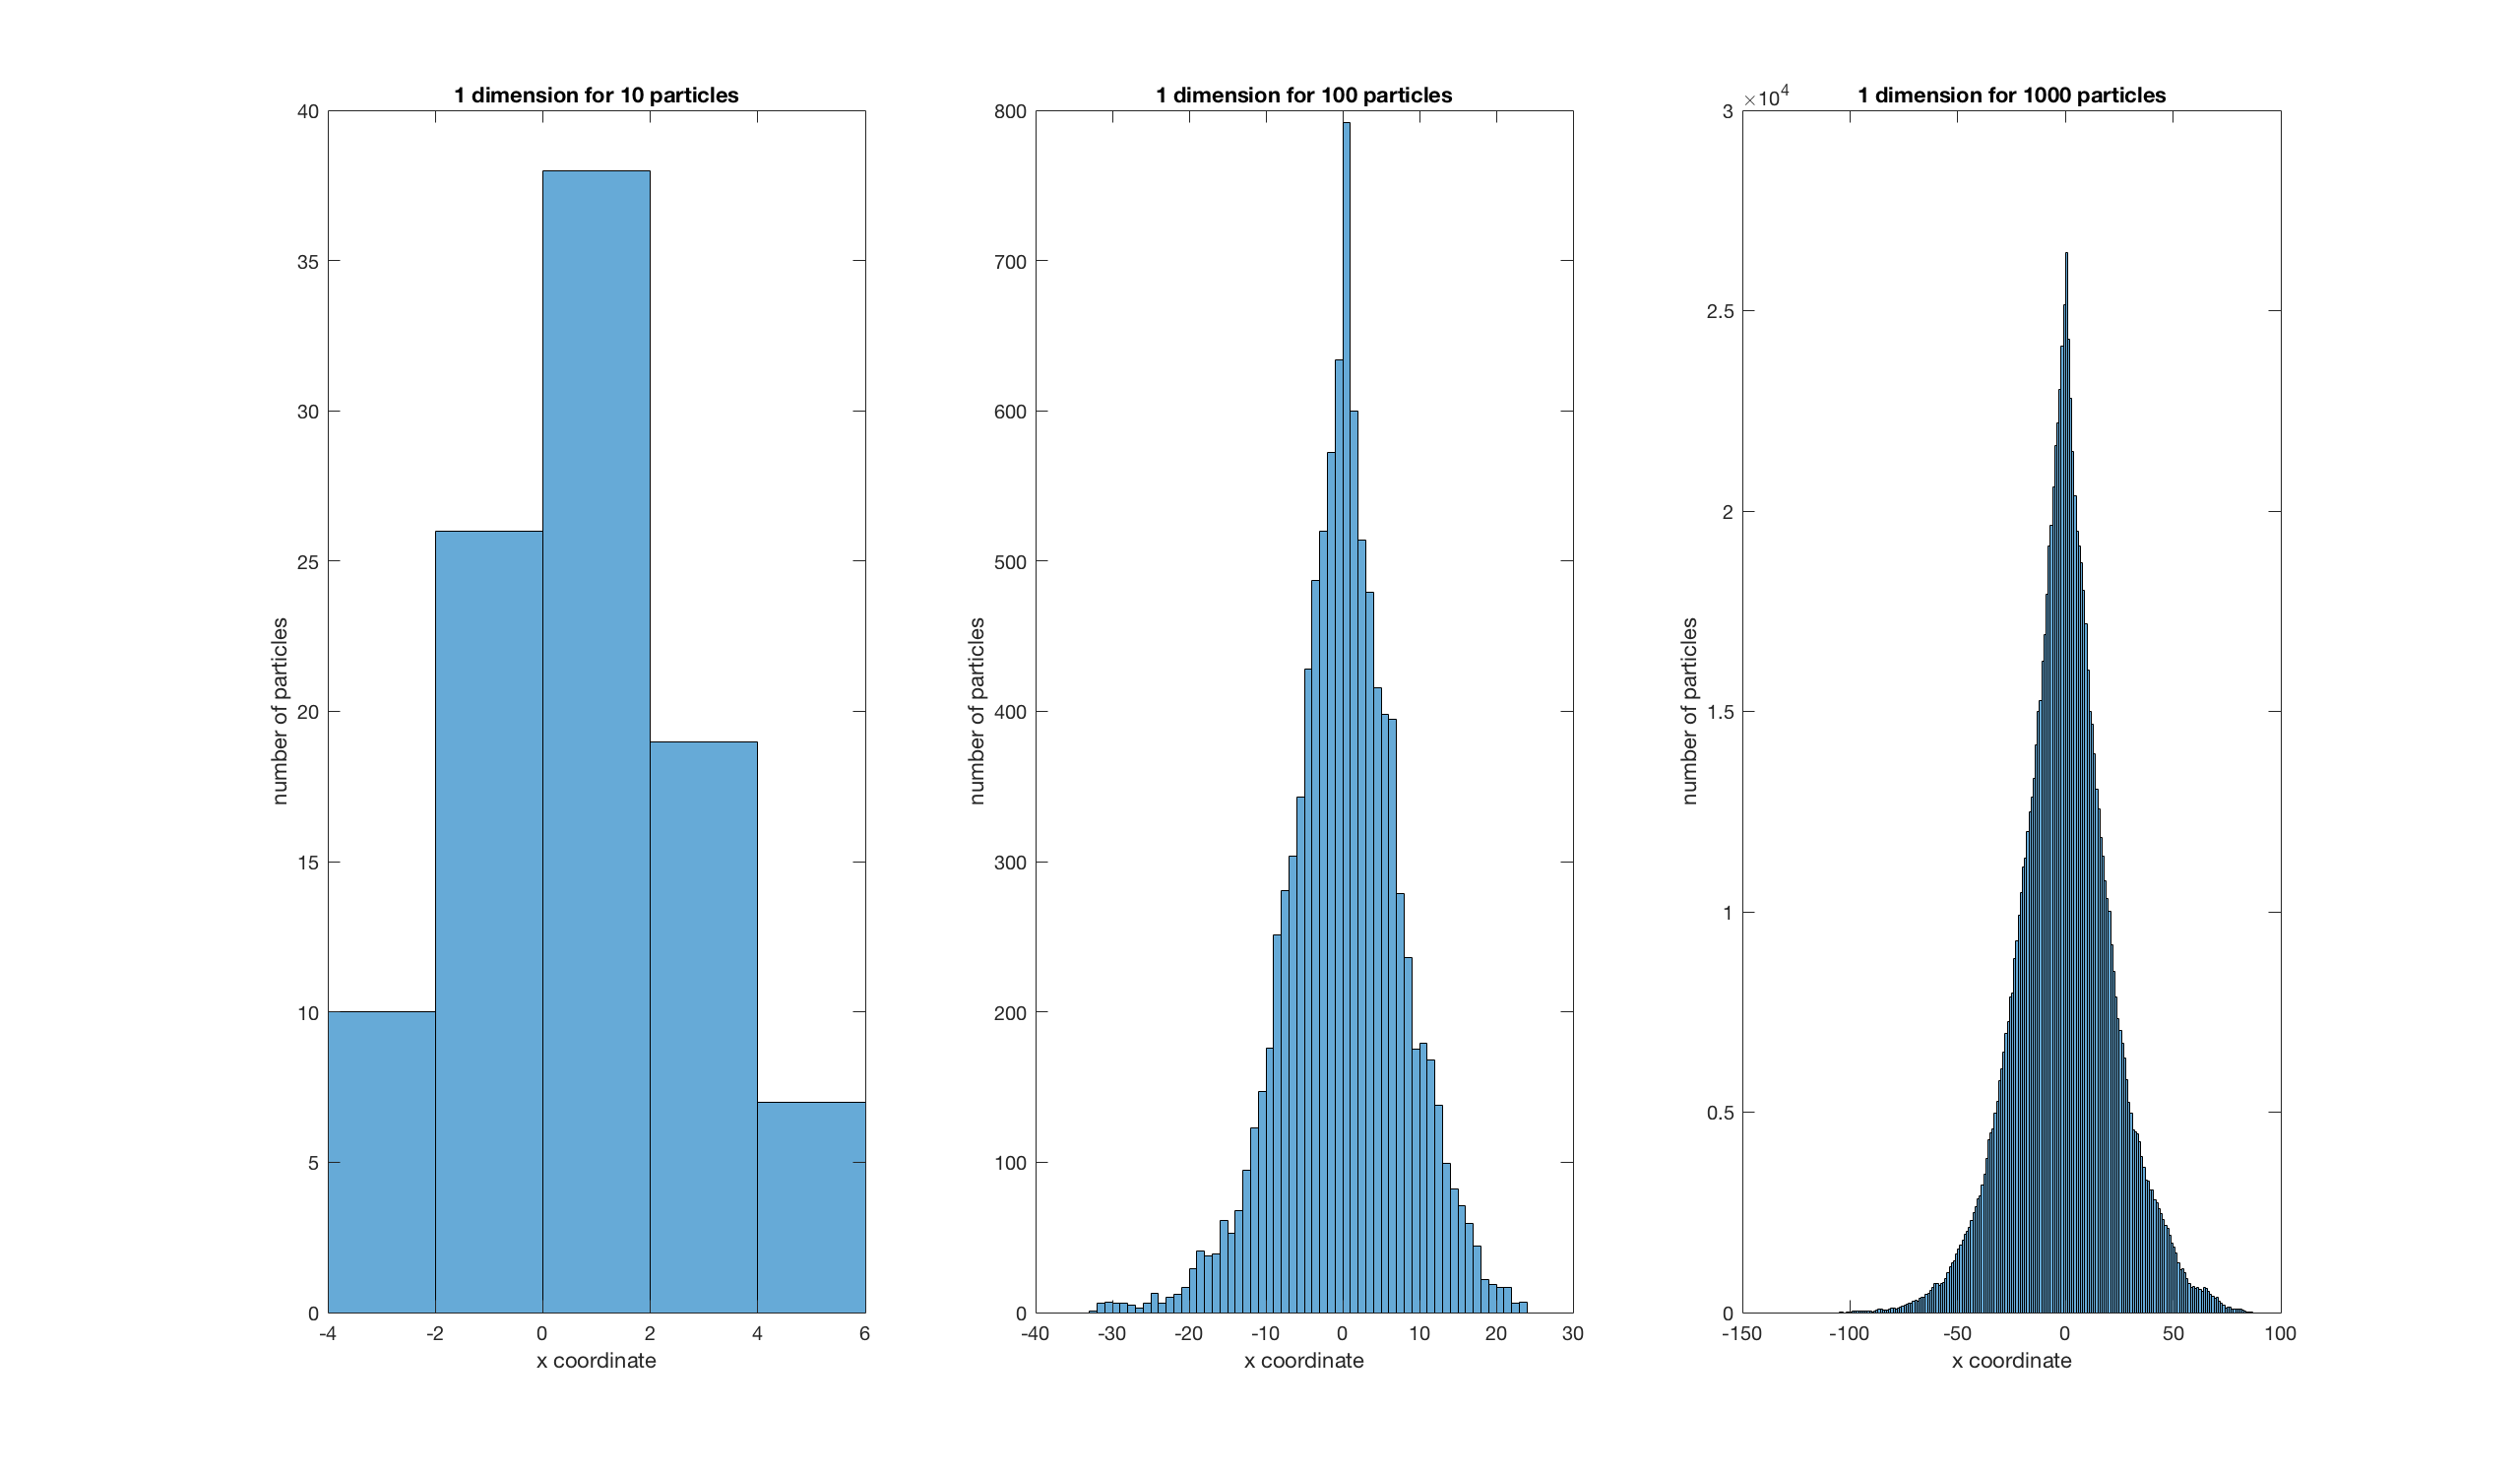
\includegraphics[width=\paperwidth,height=8cm]{hist_1d}}
\caption{Histograms of particle density evolution in 1d}
\label{fig:hist_1d}
\end{figure}

\begin{figure}[H]
\noindent\makebox[\textwidth]{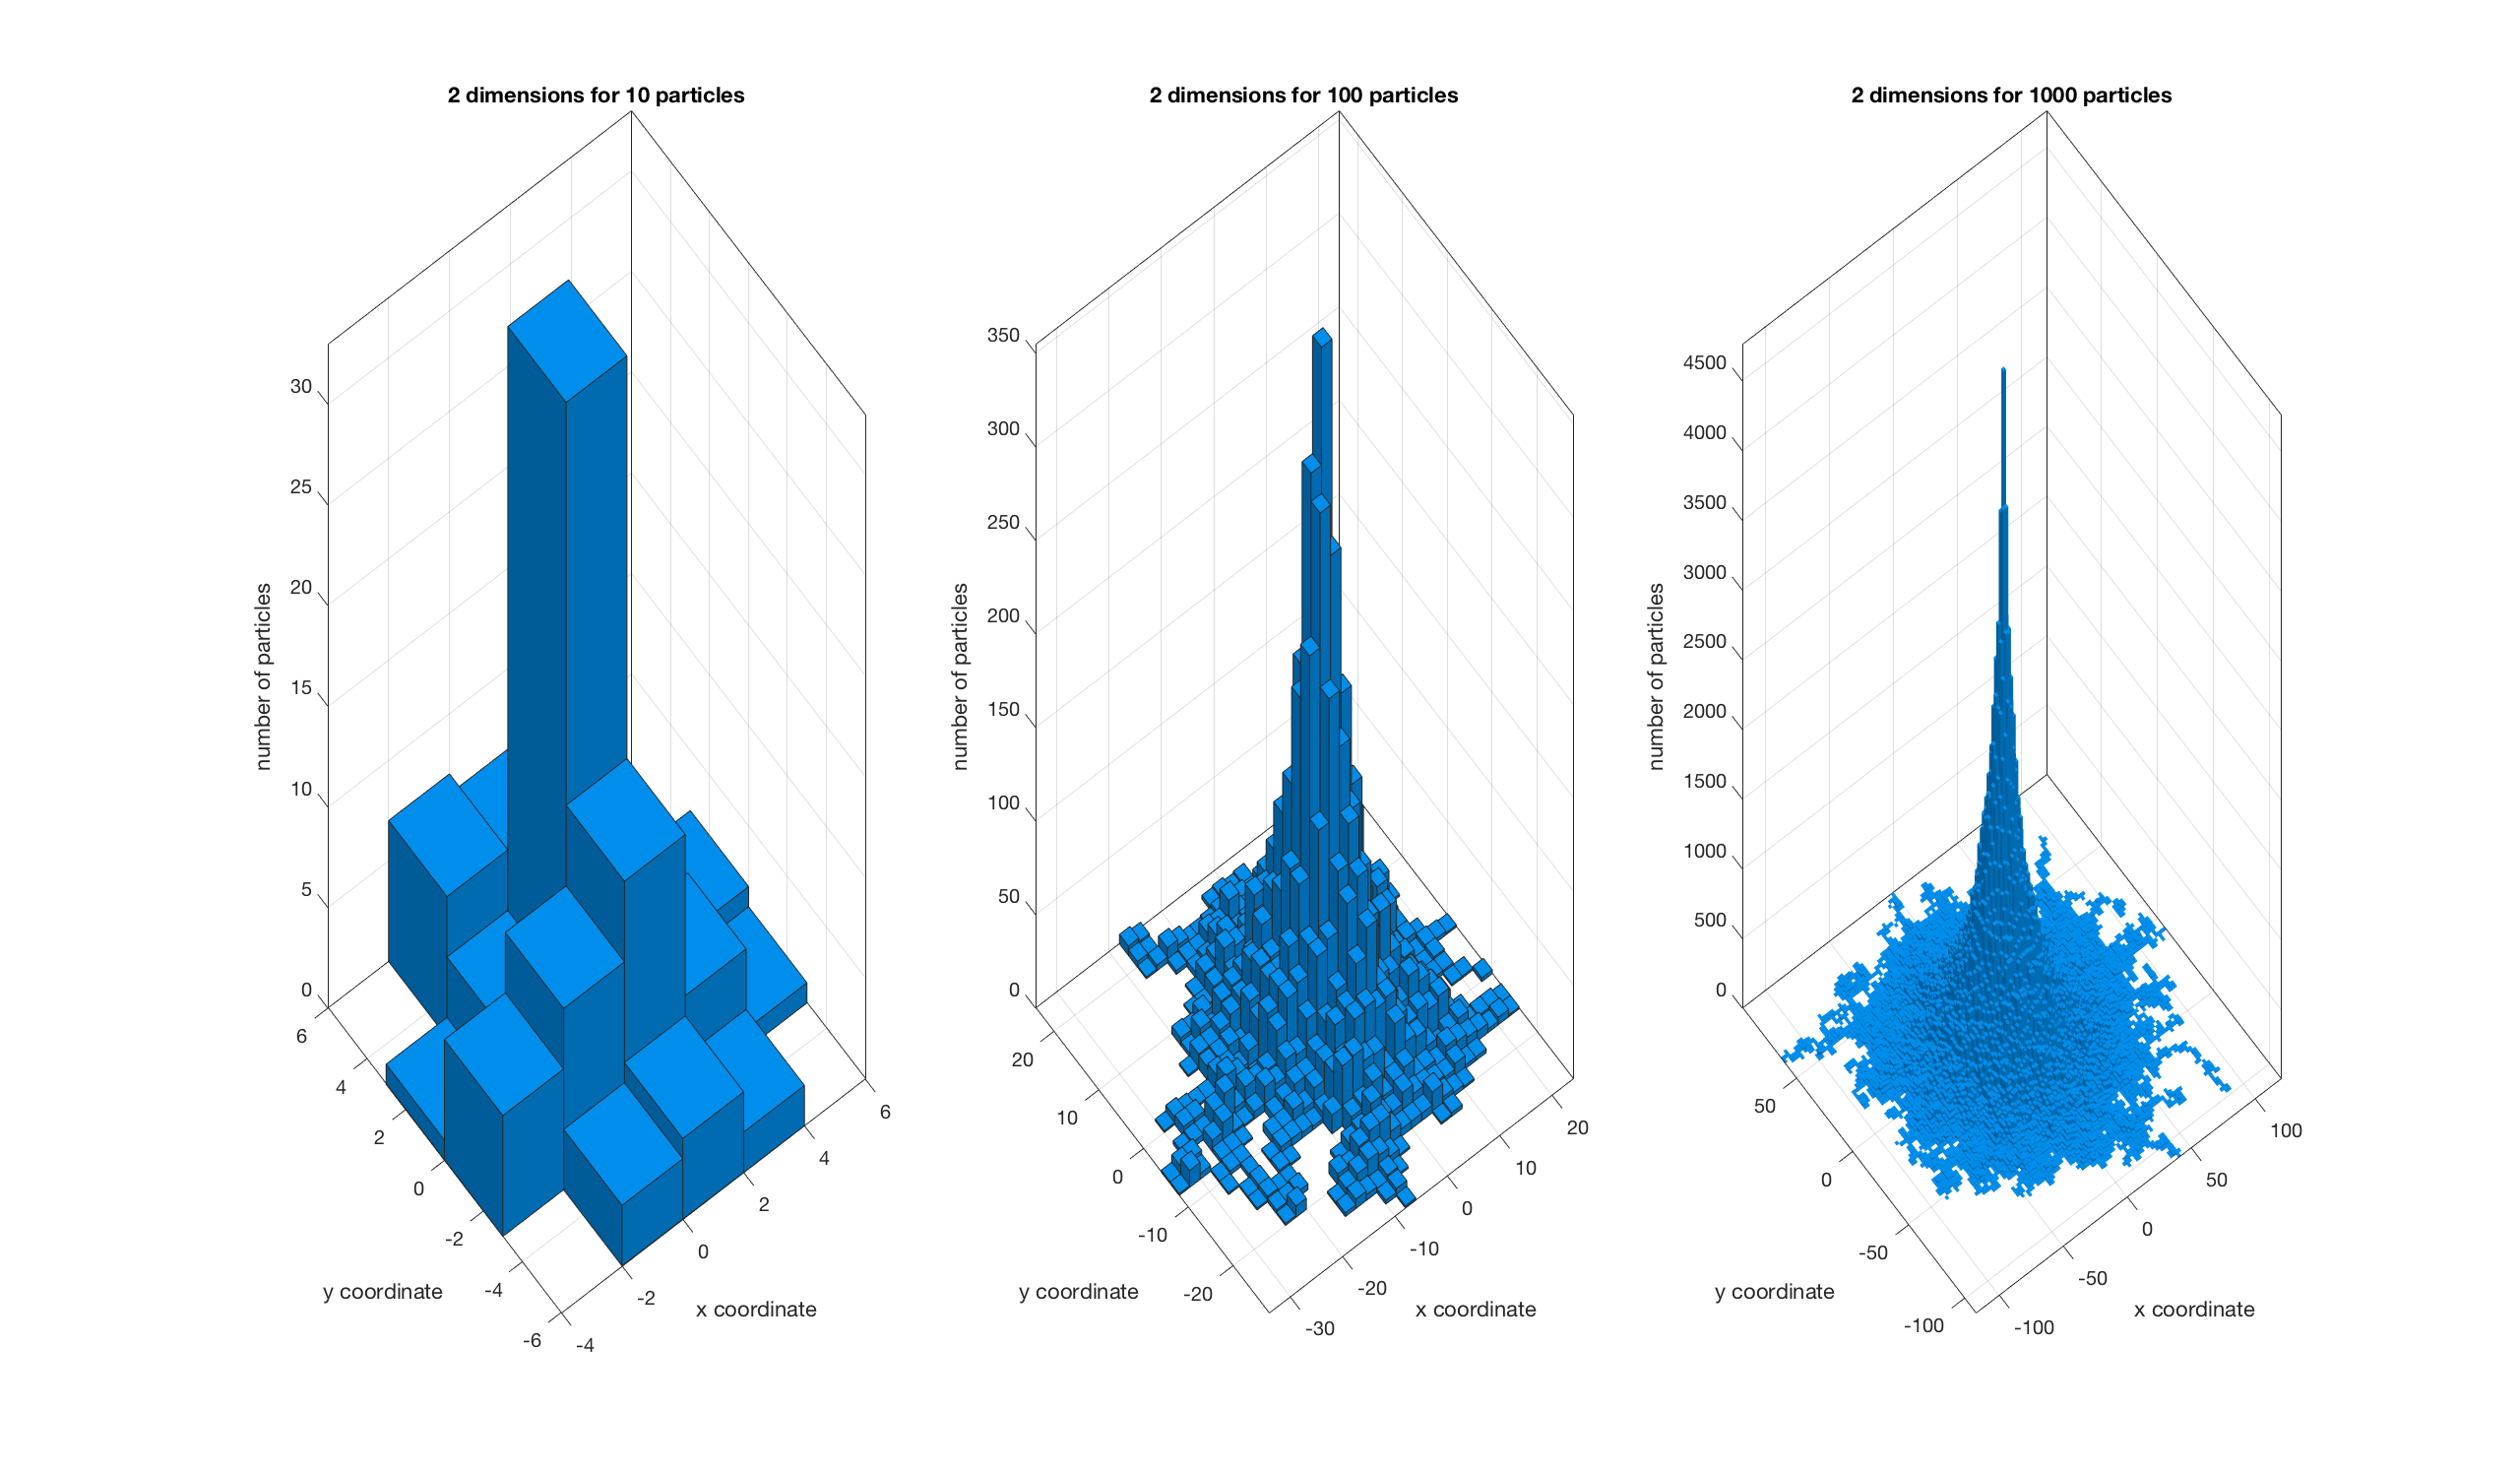
\includegraphics[width=\paperwidth,height=8cm]{hist_2d}}
\caption{Histograms of particle density evolution in 2d}
\label{fig:hist_2d}
\end{figure}

Concluding from given histograms, it can be assumed that this data seek to normal distribution (Gausian distribution) despite number of dimensions taken in to account. 


\subsection{Autocorrelation property}

To inspect autocorrelation property of Brownian motion it can be shown in comparison with autocorrelation of random data. For this purpose, simple MATLAB script were prepared, and can be read at listing \ref{lst:autocorr}

\begin{lstlisting}[language=Matlab,frame=single,label={lst:autocorr},breaklines=true,caption={Script that outputs autocorrelation for Brownian motion and random vector of data}]
figure;
rc = [];
random_values = rand(1, 1000);
for i = -50:50
    rc = [rc corr(random_values(100:900)', random_values(100+i:900+i)')];
end
plot(rc);
xlabel('random position');
ylabel('auto correlation value');
title('Auto correlation of random values');

x = [0];
for i=2:1000
   x = [x x(i-1)+randn()];
end

bc = []
for i = -50:50
    bc = [bc corr(x(100:900)', x(100+i:900+i)')];
end

figure;
plot(bc);
xlabel('random walk position');
ylabel('auto correlation value');
title('Auto correlation of Brownian motion');
\end{lstlisting}
\vspace{1em}
Output of this script can be found on figure \ref{fig:ac_r} and \ref{fig:ac_b}

\begin{figure}[H]
\noindent\makebox[\textwidth]{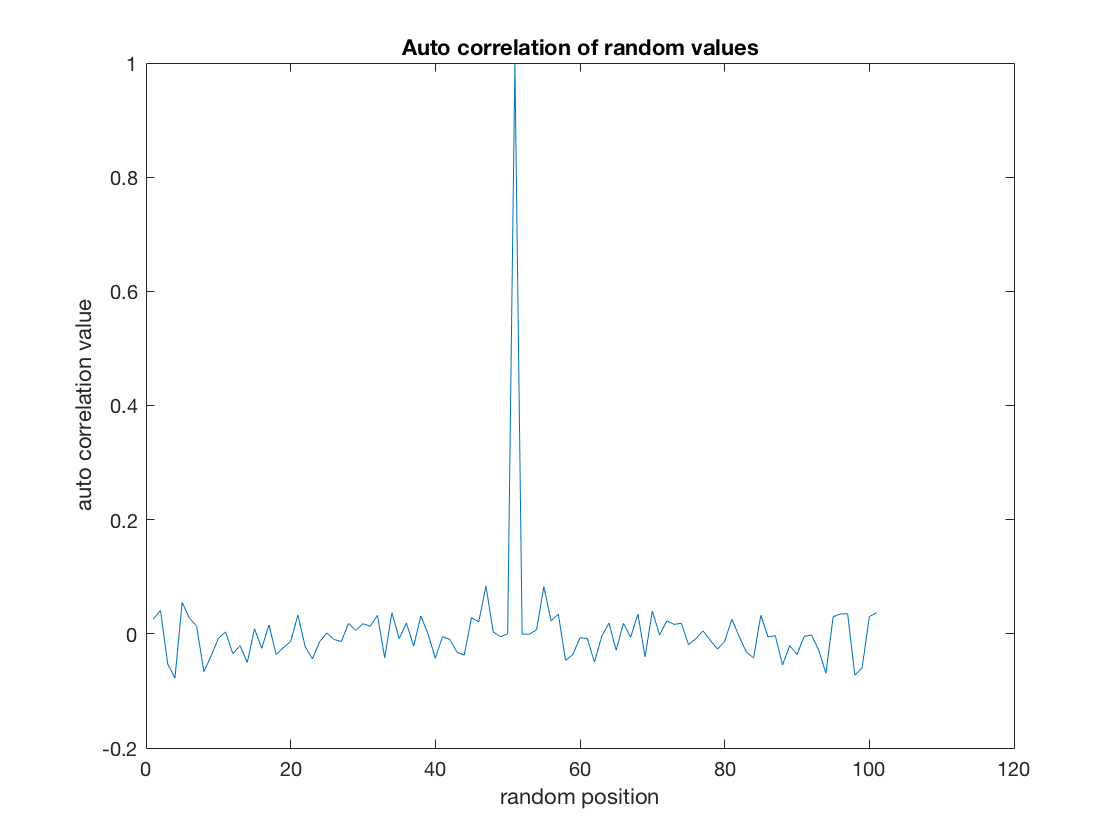
\includegraphics[width=\paperwidth,height=8cm]{ac_r}}
\caption{Autocorrelation of random vector of data}
\label{fig:ac_r}
\end{figure}

\begin{figure}[H]
\noindent\makebox[\textwidth]{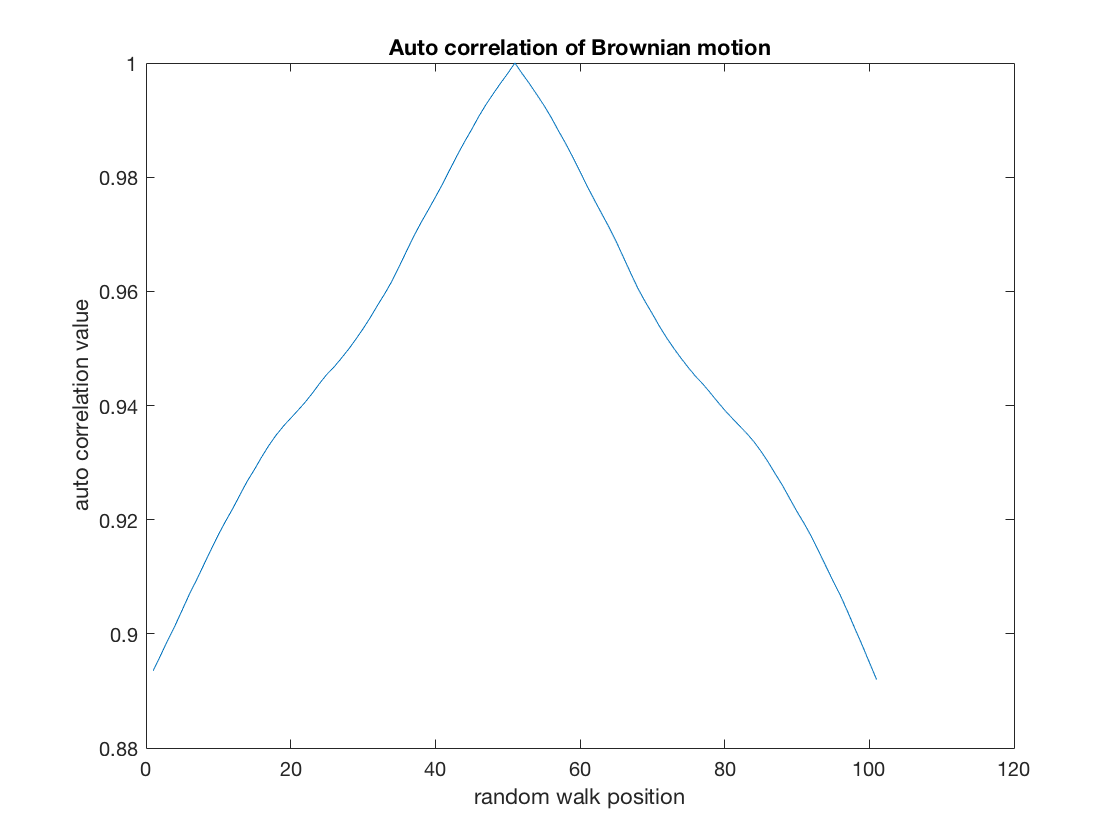
\includegraphics[width=\paperwidth,height=8cm]{ac_b}}
\caption{Autocorrelation of vector containing Brownian motion data}
\label{fig:ac_b}
\end{figure}

Comparing these two charts, it is observable that Brownian motion autocorrelation factor is much higher then random data, getting close to 1 and not dropping below 0.88. 

\section{Conclusion}
In this report Brownian motion and its properties was covered. Various matlab scripts were written to illustrate random walk itself, its square mean of displacement, time evolution of particles density and its autocorrelation property. It is called ``random'' walk, however, as the analysis shown it undergoes some well known phenomenons like normal distribution or self similarity.
\end{document}
